\section{Monodromy groups of rank 5}

\begin{figure}[H]
  \begin{center}
    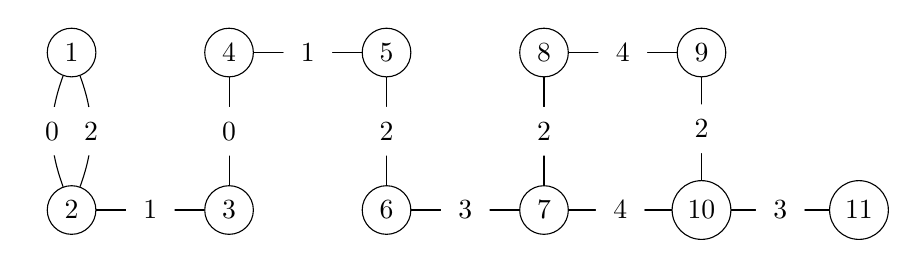
\begin{tikzpicture}

      \begin{scope}[every node/.style={circle,draw}]
        \node (1)  at (0,2)  {1};
        \node (2)  at (0,0)  {2};
        \node (3)  at (2,0)  {3};
        \node (4)  at (2,2)  {4};
        \node (5)  at (4,2)  {5};
        \node (6)  at (4,0)  {6};
        \node (7)  at (6,0)  {7};
        \node (8)  at (6,2)  {8};
        \node (9)  at (8,2)  {9};
        \node (10) at (8,0)  {10};
        \node (11) at (10,0) {11};
      \end{scope}

      \begin{scope}[every node/.style={fill=white,circle}]

        \begin{scope}[every edge/.style={draw}]
          \path (1)  edge[bend right=20] node {$0$} (2);
          \path (3)  edge node {$0$} (4);
          \path (2)  edge node {$1$} (3);
          \path (4)  edge node {$1$} (5);
          \path (1)  edge[bend left=20] node {$2$} (2);
          \path (5)  edge node {$2$} (6);
          \path (7)  edge node {$2$} (8);
          \path (9)  edge node {$2$} (10);
          \path (6)  edge node {$3$} (7);
          \path (10) edge node {$3$} (11);
          \path (7)  edge node {$4$} (10);
          \path (8)  edge node {$4$} (9);
        \end{scope}
      \end{scope}

    \end{tikzpicture}
    \caption{[1, 5, 994, 219, 267]}
  \end{center}
\end{figure}

\begin{figure}[H]
  \begin{center}
    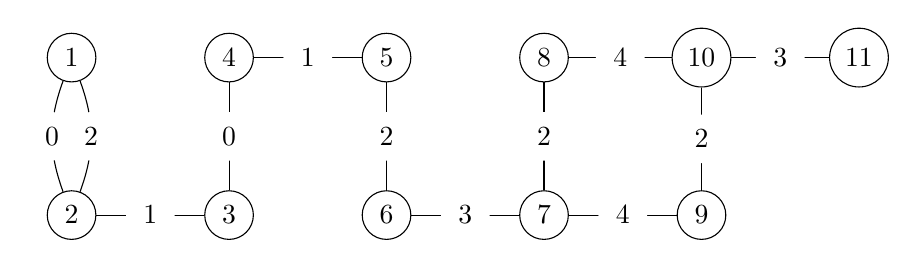
\begin{tikzpicture}

      \begin{scope}[every node/.style={circle,draw}]
        \node (1)  at (0,2)  {1};
        \node (2)  at (0,0)  {2};
        \node (3)  at (2,0)  {3};
        \node (4)  at (2,2)  {4};
        \node (5)  at (4,2)  {5};
        \node (6)  at (4,0)  {6};
        \node (7)  at (6,0)  {7};
        \node (8)  at (6,2)  {8};
        \node (9)  at (8,0)  {9};
        \node (10) at (8,2)  {10};
        \node (11) at (10,2) {11};
      \end{scope}

      \begin{scope}[every node/.style={fill=white,circle}]

        \begin{scope}[every edge/.style={draw}]
          \path (1)  edge[bend right=20] node {$0$} (2);
          \path (3)  edge node {$0$} (4);
          \path (2)  edge node {$1$} (3);
          \path (4)  edge node {$1$} (5);
          \path (1)  edge[bend left=20] node {$2$} (2);
          \path (5)  edge node {$2$} (6);
          \path (7)  edge node {$2$} (8);
          \path (9)  edge node {$2$} (10);
          \path (6)  edge node {$3$} (7);
          \path (10) edge node {$3$} (11);
          \path (7)  edge node {$4$} (9);
          \path (8)  edge node {$4$} (10);
        \end{scope}
      \end{scope}

    \end{tikzpicture}
    \caption{[1, 5, 994, 219, 381]}
  \end{center}
\end{figure}

\begin{figure}[H]
  \begin{center}
    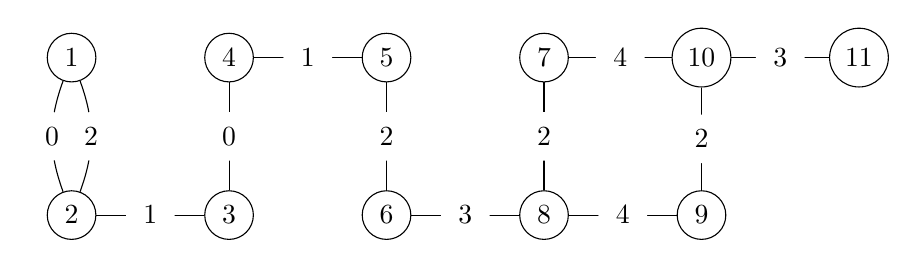
\begin{tikzpicture}

      \begin{scope}[every node/.style={circle,draw}]
        \node (1)  at (0,2)  {1};
        \node (2)  at (0,0)  {2};
        \node (3)  at (2,0)  {3};
        \node (4)  at (2,2)  {4};
        \node (5)  at (4,2)  {5};
        \node (6)  at (4,0)  {6};
        \node (7)  at (6,2)  {7};
        \node (8)  at (6,0)  {8};
        \node (9)  at (8,0)  {9};
        \node (10) at (8,2)  {10};
        \node (11) at (10,2) {11};
      \end{scope}

      \begin{scope}[every node/.style={fill=white,circle}]

        \begin{scope}[every edge/.style={draw}]
          \path (1)  edge[bend right=20] node {$0$} (2);
          \path (3)  edge node {$0$} (4);
          \path (2)  edge node {$1$} (3);
          \path (4)  edge node {$1$} (5);
          \path (1)  edge[bend left=20] node {$2$} (2);
          \path (5)  edge node {$2$} (6);
          \path (7)  edge node {$2$} (8);
          \path (9)  edge node {$2$} (10);
          \path (6)  edge node {$3$} (8);
          \path (10) edge node {$3$} (11);
          \path (7)  edge node {$4$} (10);
          \path (8)  edge node {$4$} (9);
        \end{scope}
      \end{scope}

    \end{tikzpicture}
    \caption{[1, 5, 994, 227, 267]}
  \end{center}
\end{figure}

\begin{figure}[H]
  \begin{center}
    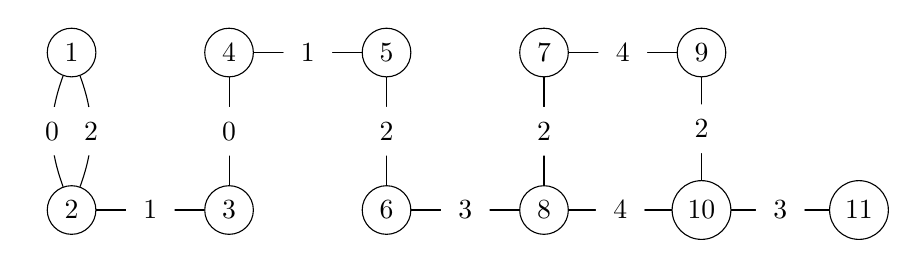
\begin{tikzpicture}

      \begin{scope}[every node/.style={circle,draw}]
        \node (1)  at (0,2)  {1};
        \node (2)  at (0,0)  {2};
        \node (3)  at (2,0)  {3};
        \node (4)  at (2,2)  {4};
        \node (5)  at (4,2)  {5};
        \node (6)  at (4,0)  {6};
        \node (7)  at (6,2)  {7};
        \node (8)  at (6,0)  {8};
        \node (9)  at (8,2)  {9};
        \node (10) at (8,0)  {10};
        \node (11) at (10,0) {11};
      \end{scope}

      \begin{scope}[every node/.style={fill=white,circle}]

        \begin{scope}[every edge/.style={draw}]
          \path (1)  edge[bend right=20] node {$0$} (2);
          \path (3)  edge node {$0$} (4);
          \path (2)  edge node {$1$} (3);
          \path (4)  edge node {$1$} (5);
          \path (1)  edge[bend left=20] node {$2$} (2);
          \path (5)  edge node {$2$} (6);
          \path (7)  edge node {$2$} (8);
          \path (9)  edge node {$2$} (10);
          \path (6)  edge node {$3$} (8);
          \path (10) edge node {$3$} (11);
          \path (7)  edge node {$4$} (9);
          \path (8)  edge node {$4$} (10);
        \end{scope}
      \end{scope}

    \end{tikzpicture}
    \caption{[1, 5, 994, 227, 381]}
  \end{center}
\end{figure}

\begin{figure}[H]
  \begin{center}
    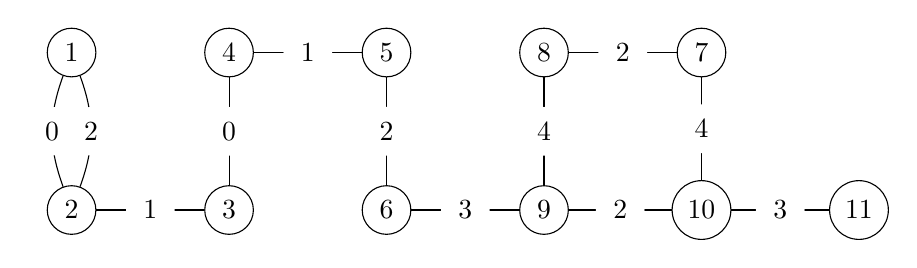
\begin{tikzpicture}

      \begin{scope}[every node/.style={circle,draw}]
        \node (1)  at (0,2)  {1};
        \node (2)  at (0,0)  {2};
        \node (3)  at (2,0)  {3};
        \node (4)  at (2,2)  {4};
        \node (5)  at (4,2)  {5};
        \node (6)  at (4,0)  {6};
        \node (7)  at (8,2)  {7};
        \node (8)  at (6,2)  {8};
        \node (9)  at (6,0)  {9};
        \node (10) at (8,0)  {10};
        \node (11) at (10,0) {11};
      \end{scope}

      \begin{scope}[every node/.style={fill=white,circle}]

        \begin{scope}[every edge/.style={draw}]
          \path (1)  edge[bend right=20] node {$0$} (2);
          \path (3)  edge node {$0$} (4);
          \path (2)  edge node {$1$} (3);
          \path (4)  edge node {$1$} (5);
          \path (1)  edge[bend left=20] node {$2$} (2);
          \path (5)  edge node {$2$} (6);
          \path (7)  edge node {$2$} (8);
          \path (9)  edge node {$2$} (10);
          \path (6)  edge node {$3$} (9);
          \path (10) edge node {$3$} (11);
          \path (7)  edge node {$4$} (10);
          \path (8)  edge node {$4$} (9);
        \end{scope}
      \end{scope}

    \end{tikzpicture}
    \caption{[1, 5, 994, 232, 267]}
  \end{center}
\end{figure}

\begin{figure}[H]
  \begin{center}
    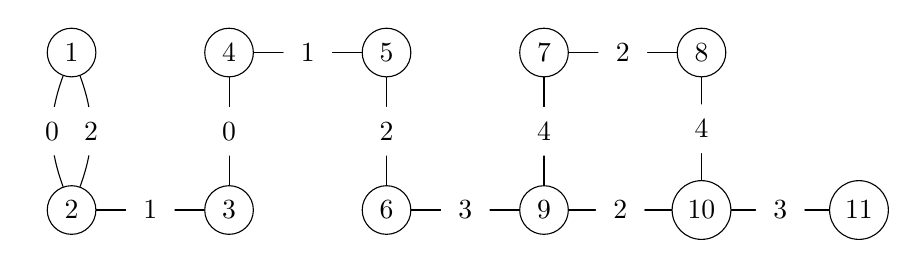
\begin{tikzpicture}

      \begin{scope}[every node/.style={circle,draw}]
        \node (1)  at (0,2)  {1};
        \node (2)  at (0,0)  {2};
        \node (3)  at (2,0)  {3};
        \node (4)  at (2,2)  {4};
        \node (5)  at (4,2)  {5};
        \node (6)  at (4,0)  {6};
        \node (7)  at (6,2)  {7};
        \node (8)  at (8,2)  {8};
        \node (9)  at (6,0)  {9};
        \node (10) at (8,0)  {10};
        \node (11) at (10,0) {11};
      \end{scope}

      \begin{scope}[every node/.style={fill=white,circle}]

        \begin{scope}[every edge/.style={draw}]
          \path (1)  edge[bend right=20] node {$0$} (2);
          \path (3)  edge node {$0$} (4);
          \path (2)  edge node {$1$} (3);
          \path (4)  edge node {$1$} (5);
          \path (1)  edge[bend left=20] node {$2$} (2);
          \path (5)  edge node {$2$} (6);
          \path (7)  edge node {$2$} (8);
          \path (9)  edge node {$2$} (10);
          \path (6)  edge node {$3$} (9);
          \path (10) edge node {$3$} (11);
          \path (7)  edge node {$4$} (9);
          \path (8)  edge node {$4$} (10);
        \end{scope}
      \end{scope}

    \end{tikzpicture}
    \caption{[1, 5, 994, 232, 381]}
  \end{center}
\end{figure}

\begin{figure}[H]
  \begin{center}
    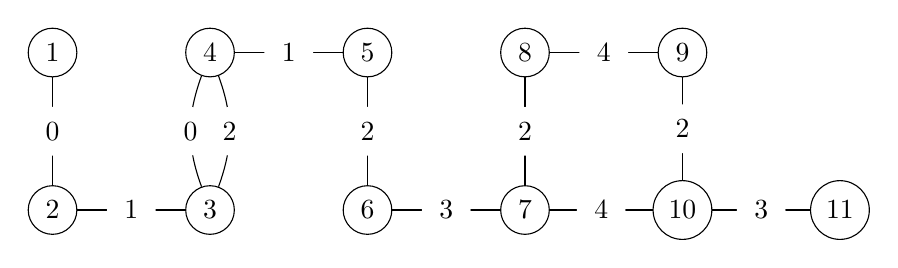
\begin{tikzpicture}

      \begin{scope}[every node/.style={circle,draw}]
        \node (1)  at (0,2)  {1};
        \node (2)  at (0,0)  {2};
        \node (3)  at (2,0)  {3};
        \node (4)  at (2,2)  {4};
        \node (5)  at (4,2)  {5};
        \node (6)  at (4,0)  {6};
        \node (7)  at (6,0)  {7};
        \node (8)  at (6,2)  {8};
        \node (9)  at (8,2)  {9};
        \node (10) at (8,0)  {10};
        \node (11) at (10,0) {11};
      \end{scope}

      \begin{scope}[every node/.style={fill=white,circle}]

        \begin{scope}[every edge/.style={draw}]
          \path (1)  edge node {$0$} (2);
          \path (3)  edge[bend left=20] node {$0$} (4);
          \path (2)  edge node {$1$} (3);
          \path (4)  edge node {$1$} (5);
          \path (3)  edge[bend right=20] node {$2$} (4);
          \path (5)  edge node {$2$} (6);
          \path (7)  edge node {$2$} (8);
          \path (9)  edge node {$2$} (10);
          \path (6)  edge node {$3$} (7);
          \path (10) edge node {$3$} (11);
          \path (7)  edge node {$4$} (10);
          \path (8)  edge node {$4$} (9);
        \end{scope}
      \end{scope}

    \end{tikzpicture}
    \caption{[1, 5, 1010, 219, 267]}
  \end{center}
\end{figure}

\begin{figure}[H]
  \begin{center}
    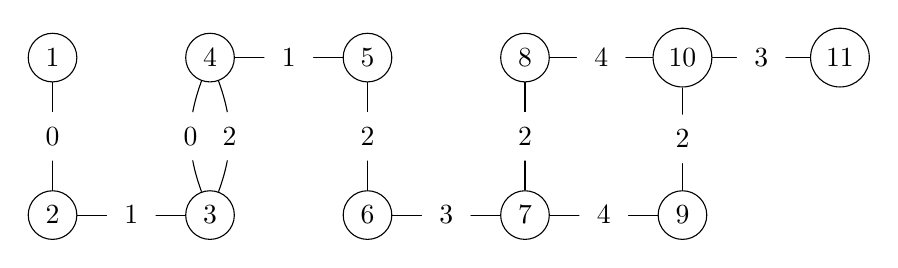
\begin{tikzpicture}

      \begin{scope}[every node/.style={circle,draw}]
        \node (1)  at (0,2)  {1};
        \node (2)  at (0,0)  {2};
        \node (3)  at (2,0)  {3};
        \node (4)  at (2,2)  {4};
        \node (5)  at (4,2)  {5};
        \node (6)  at (4,0)  {6};
        \node (7)  at (6,0)  {7};
        \node (8)  at (6,2)  {8};
        \node (9)  at (8,0)  {9};
        \node (10) at (8,2)  {10};
        \node (11) at (10,2) {11};
      \end{scope}

      \begin{scope}[every node/.style={fill=white,circle}]

        \begin{scope}[every edge/.style={draw}]
          \path (1)  edge node {$0$} (2);
          \path (3)  edge[bend left=20] node {$0$} (4);
          \path (2)  edge node {$1$} (3);
          \path (4)  edge node {$1$} (5);
          \path (3)  edge[bend right=20] node {$2$} (4);
          \path (5)  edge node {$2$} (6);
          \path (7)  edge node {$2$} (8);
          \path (9)  edge node {$2$} (10);
          \path (6)  edge node {$3$} (7);
          \path (10) edge node {$3$} (11);
          \path (7)  edge node {$4$} (9);
          \path (8)  edge node {$4$} (10);
        \end{scope}
      \end{scope}

    \end{tikzpicture}
    \caption{[1, 5, 1010, 219, 381]}
  \end{center}
\end{figure}

\begin{figure}[H]
  \begin{center}
    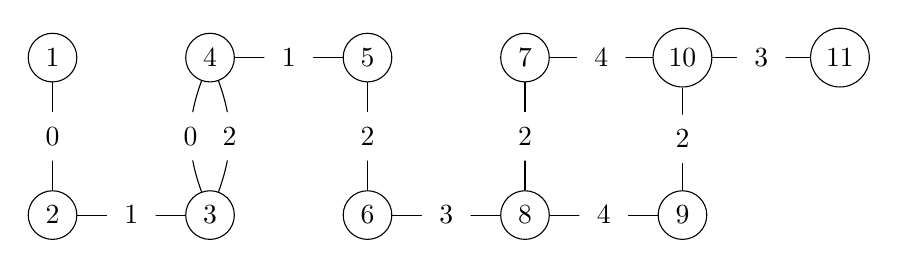
\begin{tikzpicture}

      \begin{scope}[every node/.style={circle,draw}]
        \node (1)  at (0,2)  {1};
        \node (2)  at (0,0)  {2};
        \node (3)  at (2,0)  {3};
        \node (4)  at (2,2)  {4};
        \node (5)  at (4,2)  {5};
        \node (6)  at (4,0)  {6};
        \node (7)  at (6,2)  {7};
        \node (8)  at (6,0)  {8};
        \node (9)  at (8,0)  {9};
        \node (10) at (8,2)  {10};
        \node (11) at (10,2) {11};
      \end{scope}

      \begin{scope}[every node/.style={fill=white,circle}]

        \begin{scope}[every edge/.style={draw}]
          \path (1)  edge node {$0$} (2);
          \path (3)  edge[bend left=20] node {$0$} (4);
          \path (2)  edge node {$1$} (3);
          \path (4)  edge node {$1$} (5);
          \path (3)  edge[bend right=20] node {$2$} (4);
          \path (5)  edge node {$2$} (6);
          \path (7)  edge node {$2$} (8);
          \path (9)  edge node {$2$} (10);
          \path (6)  edge node {$3$} (8);
          \path (10) edge node {$3$} (11);
          \path (7)  edge node {$4$} (10);
          \path (8)  edge node {$4$} (9);
        \end{scope}
      \end{scope}

    \end{tikzpicture}
    \caption{[1, 5, 1010, 227, 267]}
  \end{center}
\end{figure}

\begin{figure}[H]
  \begin{center}
    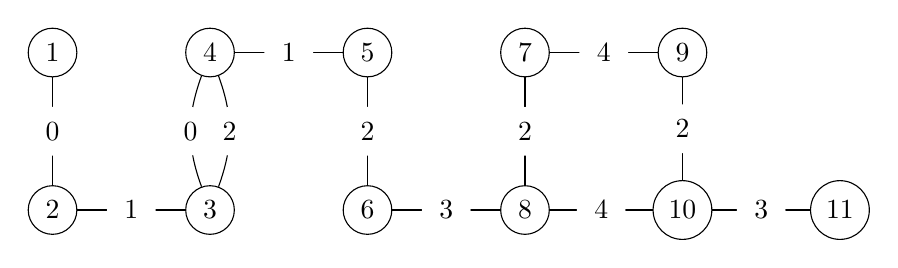
\begin{tikzpicture}

      \begin{scope}[every node/.style={circle,draw}]
        \node (1)  at (0,2)  {1};
        \node (2)  at (0,0)  {2};
        \node (3)  at (2,0)  {3};
        \node (4)  at (2,2)  {4};
        \node (5)  at (4,2)  {5};
        \node (6)  at (4,0)  {6};
        \node (7)  at (6,2)  {7};
        \node (8)  at (6,0)  {8};
        \node (9)  at (8,2)  {9};
        \node (10) at (8,0)  {10};
        \node (11) at (10,0) {11};
      \end{scope}

      \begin{scope}[every node/.style={fill=white,circle}]

        \begin{scope}[every edge/.style={draw}]
          \path (1)  edge node {$0$} (2);
          \path (3)  edge[bend left=20] node {$0$} (4);
          \path (2)  edge node {$1$} (3);
          \path (4)  edge node {$1$} (5);
          \path (3)  edge[bend right=20] node {$2$} (4);
          \path (5)  edge node {$2$} (6);
          \path (7)  edge node {$2$} (8);
          \path (9)  edge node {$2$} (10);
          \path (6)  edge node {$3$} (8);
          \path (10) edge node {$3$} (11);
          \path (7)  edge node {$4$} (9);
          \path (8)  edge node {$4$} (10);
        \end{scope}
      \end{scope}

    \end{tikzpicture}
    \caption{[1, 5, 1010, 227, 381]}
  \end{center}
\end{figure}

\begin{figure}[H]
  \begin{center}
    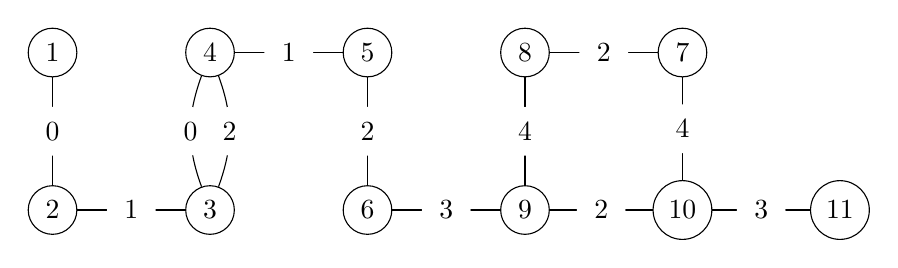
\begin{tikzpicture}

      \begin{scope}[every node/.style={circle,draw}]
        \node (1)  at (0,2)  {1};
        \node (2)  at (0,0)  {2};
        \node (3)  at (2,0)  {3};
        \node (4)  at (2,2)  {4};
        \node (5)  at (4,2)  {5};
        \node (6)  at (4,0)  {6};
        \node (7)  at (8,2)  {7};
        \node (8)  at (6,2)  {8};
        \node (9)  at (6,0)  {9};
        \node (10) at (8,0)  {10};
        \node (11) at (10,0) {11};
      \end{scope}

      \begin{scope}[every node/.style={fill=white,circle}]

        \begin{scope}[every edge/.style={draw}]
          \path (1)  edge node {$0$} (2);
          \path (3)  edge[bend left=20] node {$0$} (4);
          \path (2)  edge node {$1$} (3);
          \path (4)  edge node {$1$} (5);
          \path (3)  edge[bend right=20] node {$2$} (4);
          \path (5)  edge node {$2$} (6);
          \path (7)  edge node {$2$} (8);
          \path (9)  edge node {$2$} (10);
          \path (6)  edge node {$3$} (9);
          \path (10) edge node {$3$} (11);
          \path (7)  edge node {$4$} (10);
          \path (8)  edge node {$4$} (9);
        \end{scope}
      \end{scope}

    \end{tikzpicture}
    \caption{[1, 5, 1010, 232, 267]}
  \end{center}
\end{figure}

\begin{figure}[H]
  \begin{center}
    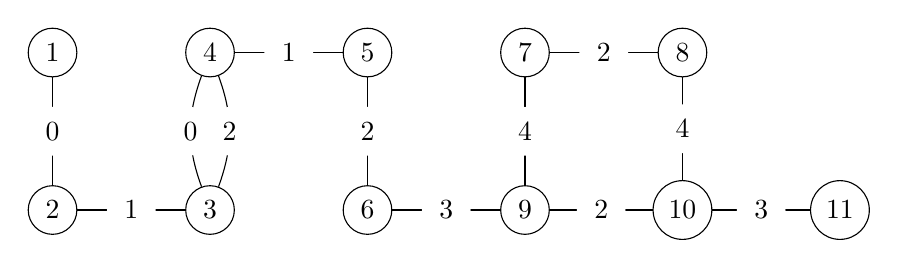
\begin{tikzpicture}

      \begin{scope}[every node/.style={circle,draw}]
        \node (1)  at (0,2)  {1};
        \node (2)  at (0,0)  {2};
        \node (3)  at (2,0)  {3};
        \node (4)  at (2,2)  {4};
        \node (5)  at (4,2)  {5};
        \node (6)  at (4,0)  {6};
        \node (7)  at (6,2)  {7};
        \node (8)  at (8,2)  {8};
        \node (9)  at (6,0)  {9};
        \node (10) at (8,0)  {10};
        \node (11) at (10,0) {11};
      \end{scope}

      \begin{scope}[every node/.style={fill=white,circle}]

        \begin{scope}[every edge/.style={draw}]
          \path (1)  edge node {$0$} (2);
          \path (3)  edge[bend left=20] node {$0$} (4);
          \path (2)  edge node {$1$} (3);
          \path (4)  edge node {$1$} (5);
          \path (3)  edge[bend right=20] node {$2$} (4);
          \path (5)  edge node {$2$} (6);
          \path (7)  edge node {$2$} (8);
          \path (9)  edge node {$2$} (10);
          \path (6)  edge node {$3$} (9);
          \path (10) edge node {$3$} (11);
          \path (7)  edge node {$4$} (9);
          \path (8)  edge node {$4$} (10);
        \end{scope}
      \end{scope}

    \end{tikzpicture}
    \caption{[1, 5, 1010, 232, 381]}
  \end{center}
\end{figure}
